\documentclass{standalone}
\usepackage{tikz}
\usetikzlibrary{decorations.pathreplacing}
\usepackage{graphicx}
\begin{document}
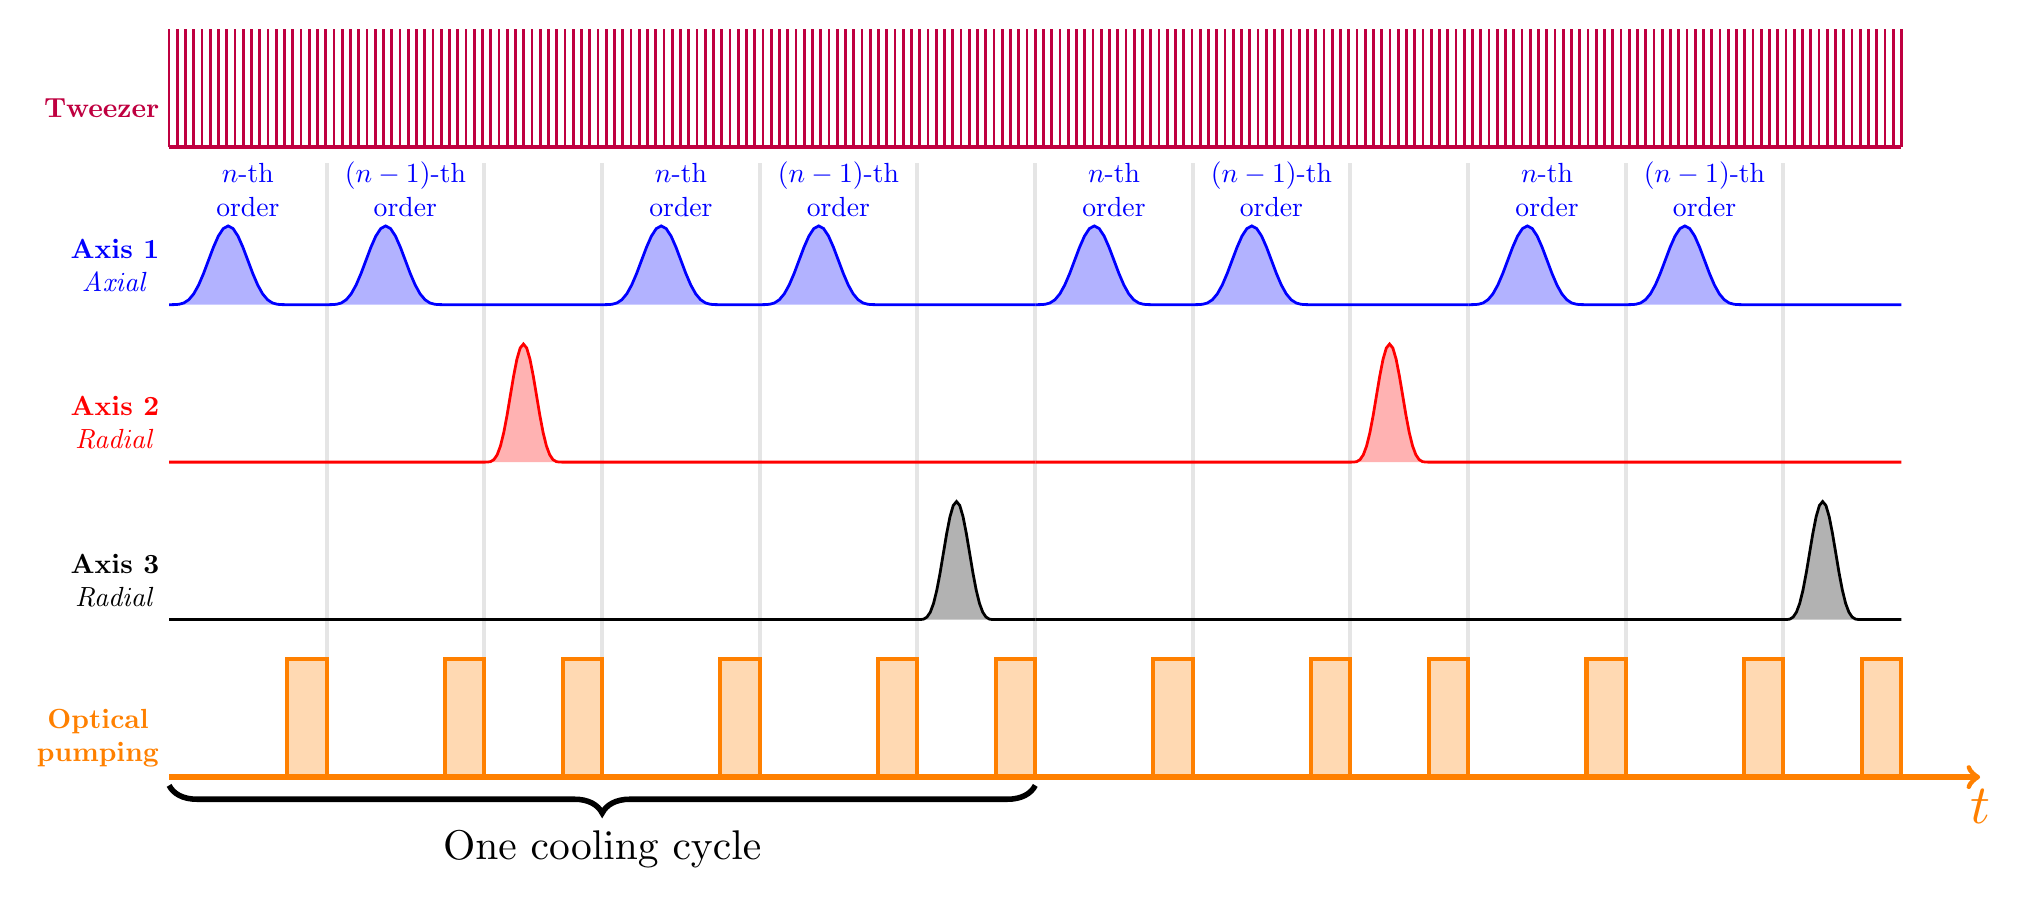
\begin{tikzpicture}
  % 0.0 - 1.5 axial
  % 1.5 - 2.0 OP
  % 2.0 - 3.5 axial
  % 3.5 - 4.0 OP
  % 4.0 - 5.0 radial 2
  % 5.0 - 5.5 OP
  % 5.5 - 7.0 axial
  % 7.0 - 7.5 OP
  % 7.5 - 9.0 axial
  % 9.0 - 9.5 OP
  % 9.5 - 10.5 radial 3
  % 10.5 - 11.0 OP

  %% Pulse mark
  \foreach \i in {2.0, 4.0, 5.5, 7.5, 9.5, 11.0, 13.0, 15.0, 16.5, 18.5, 20.5} {
    \draw[gray!20, line width=1.5] (\i, 1.8) -- (\i, -6.0);
  }

  %% Tweezer
  \draw[line width=1.5,purple] (0, 2) -- (22, 2);
  \foreach \i in {0,...,210} {
    \draw[line width=1,purple] (\i*22/210, 2) -- (\i*22/210, 3.5);
  }
  \path (0, 2.5) node[left,purple,align=center] {\textbf{Tweezer}};

  %% Axial
  \foreach \i in {0, 5.5, 11.0, 16.5} {
    \fill[blue!30]
    plot[draw,samples=200,domain=\i:{\i+1.5},variable=\x] ({\x}, {sin((\x-\i) * 120)^4})
    -- cycle;
    \path (\i+1, 1) node[above,blue,align=center] {$n$-th\\order};
    \fill[blue!30]
    plot[draw,samples=200,domain={\i+2.0}:{\i+3.5},variable=\x] ({\x}, {sin((\x-\i-2.0) * 120)^4})
    -- cycle;
    \path (\i+3, 1) node[above,blue,align=center] {$(n-1)$-th\\order};
    \draw[line width=1,blue] plot[domain=\i:{\i+1.5},variable=\x]
    ({\x}, {sin((\x-\i) * 120)^4}) -- (\i+2.0, 0)
    plot[domain={\i+2.0}:{\i+3.5},variable=\x]
    ({\x}, {sin((\x-\i-2.0) * 120)^4})-- (\i+5.5, 0);
  }
  \path (0, 0.5) node[left,blue,align=center] {\textbf{Axis 1}\\\textit{Axial}};

  %% Radial 2
  \foreach \i in {0, 11.0} {
    \fill[red!30]
    plot[draw,samples=200,domain={\i+4.0}:{\i+5.0},variable=\x] ({\x}, {1.5*sin((\x-\i-4.0) * 180)^4 - 2})
    -- cycle;
    \draw[line width=1,red] (\i, -2) -- plot[domain={\i+4.0}:{\i+5.0},variable=\x]
    ({\x}, {1.5*sin((\x-\i-4.0) * 180)^4 - 2}) -- (\i+11.0, -2);
  }
  \path (0, -1.5) node[left,red,align=center] {\textbf{Axis 2}\\\textit{Radial}};

  %% Radial 3
  \foreach \i in {0, 11.0} {
    \fill[black!30]
    plot[draw,samples=200,domain={\i+9.5}:{\i+10.5},variable=\x] ({\x}, {1.5*sin((\x-\i-9.5) * 180)^4 - 4})
    -- cycle;
    \draw[line width=1,black] (\i, -4) -- plot[domain={\i+9.5}:{\i+10.5},variable=\x]
    ({\x}, {1.5*sin((\x-\i-9.5) * 180)^4 - 4}) -- (\i+11.0, -4);
  }
  \path (0, -3.5) node[left,black,align=center] {\textbf{Axis 3}\\\textit{Radial}};

  %% OP
  \foreach \i in {0, 5.5, 11.0, 16.5} {
    \filldraw[fill=orange!30,draw=orange,line width=1.5]
    (\i+1.5, -6) -- (\i+1.5, -4.5) -- (\i+2.0, -4.5) -- (\i+2.0, -6) -- cycle;
    \filldraw[fill=orange!30,draw=orange,line width=1.5]
    (\i+3.5, -6) -- (\i+3.5, -4.5) -- (\i+4.0, -4.5) -- (\i+4.0, -6) -- cycle;
    \filldraw[fill=orange!30,draw=orange,line width=1.5]
    (\i+5.0, -6) -- (\i+5.0, -4.5) -- (\i+5.5, -4.5) -- (\i+5.5, -6) -- cycle;
  }
  \path (0, -5.5) node[left,orange,align=center] {\textbf{Optical}\\\textbf{pumping}};
  \draw[line width=2,orange,->] (0,-6) -- (23,-6) node[right, below] {\scalebox{2}{$t$}};

  %% Cycle mark
  \draw[decoration={brace,mirror,raise=3pt, amplitude=10pt},decorate,line width=2]
  (0,-6) -- node[below=15pt] {\scalebox{1.5}{One cooling cycle}} (11,-6);
\end{tikzpicture}
\end{document}
